\documentclass[11pt,a4paper]{article}

\usepackage[a4paper,landscape,margin=13mm]{geometry}
\usepackage[T1]{fontenc}
\usepackage[utf8]{inputenc}
\usepackage[english]{babel}
\usepackage{lmodern}
\usepackage{booktabs}
\usepackage{xcolor}
\usepackage{pgfplots}
\usepackage{amsmath}

\renewcommand{\familydefault}{\sfdefault}
\pgfplotsset{compat=1.18}
\pagestyle{empty}
\setlength{\parindent}{0pt}
\setlength{\parskip}{0.35em}

\definecolor{dmblue}{HTML}{3F7DF1}
\definecolor{goodgreen}{HTML}{209B3A}
\definecolor{linegray}{HTML}{AEB4BE}

\newcommand{\initAWin}{0.008}
\newcommand{\initBWin}{0.084}
\newcommand{\initTie}{0.908}
\newcommand{\crossAWin}{0.340}
\newcommand{\crossBWin}{0.516}
\newcommand{\crossTie}{0.144}
\newcommand{\crossAReward}{0.1429}
\newcommand{\crossBReward}{0.1721}

\newcommand{\selfQwenWin}{0.285}
\newcommand{\selfQwenReward}{0.083}
\newcommand{\selfSmolWin}{0.465}
\newcommand{\selfSmolReward}{0.132}

\newcommand{\PanelTitle}[1]{{\Large\bfseries\color{dmblue}#1}\par\vspace{0.18em}}

\begin{document}

{\Huge\bfseries\color{dmblue}CrossPlay and Self-Play Results}\hfill
{\large Qwen2.5-0.5B-Instruct / SmolLM2-1.7B-Instruct on GSM8K}

\vspace{0.5em}
{\color{linegray}\rule{\linewidth}{1pt}}
\vspace{0.9em}

\begin{minipage}[t]{0.32\linewidth}
\PanelTitle{1. CrossPlay}
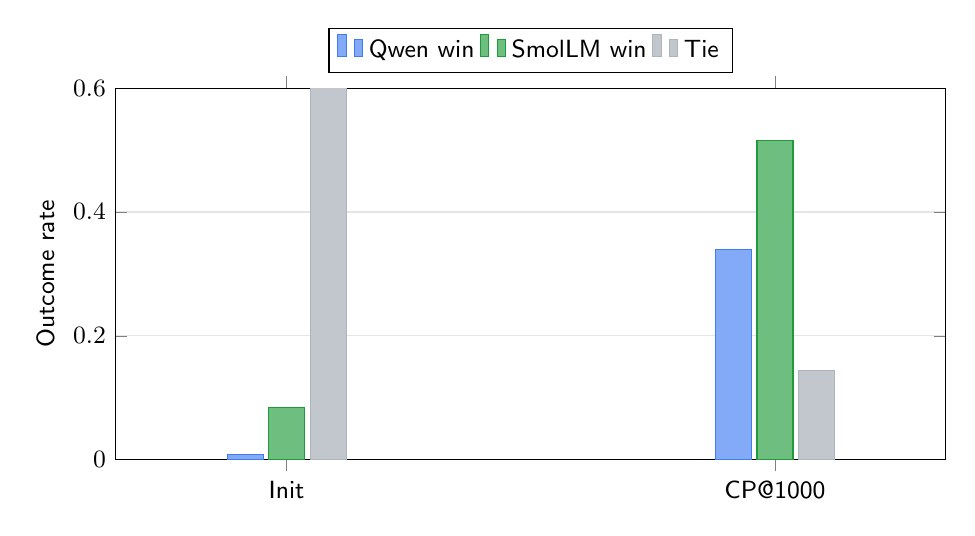
\begin{tikzpicture}
\begin{axis}[
  width=\linewidth,
  height=63mm,
  ybar,
  bar width=13pt,
  ymin=0,
  ymax=0.60,
  symbolic x coords={Init,CP@1000},
  xtick=data,
  ylabel={Outcome rate},
  tick label style={font=\small},
  ylabel style={font=\small},
  legend style={font=\small,at={(0.5,1.04)},anchor=south,legend columns=3},
  ymajorgrids=true,
  grid style={linegray!35},
  enlarge x limits=0.35
]
\addplot+[fill=dmblue!65,draw=dmblue] coordinates {(Init,\initAWin) (CP@1000,\crossAWin)};
\addplot+[fill=goodgreen!65,draw=goodgreen] coordinates {(Init,\initBWin) (CP@1000,\crossBWin)};
\addplot+[fill=linegray!75,draw=linegray] coordinates {(Init,\initTie) (CP@1000,\crossTie)};
\legend{Qwen win,SmolLM win,Tie}
\end{axis}
\end{tikzpicture}

\vspace{0.3em}
\begin{tabular}{@{}lccc@{}}
\toprule
Run & Qwen & SmolLM & Tie \\
\midrule
Init & \initAWin & \initBWin & \initTie \\
CP@1000 & \crossAWin & \crossBWin & \crossTie \\
\bottomrule
\end{tabular}
\end{minipage}
\hfill
\begin{minipage}[t]{0.32\linewidth}
\PanelTitle{2. Qwen self-play}
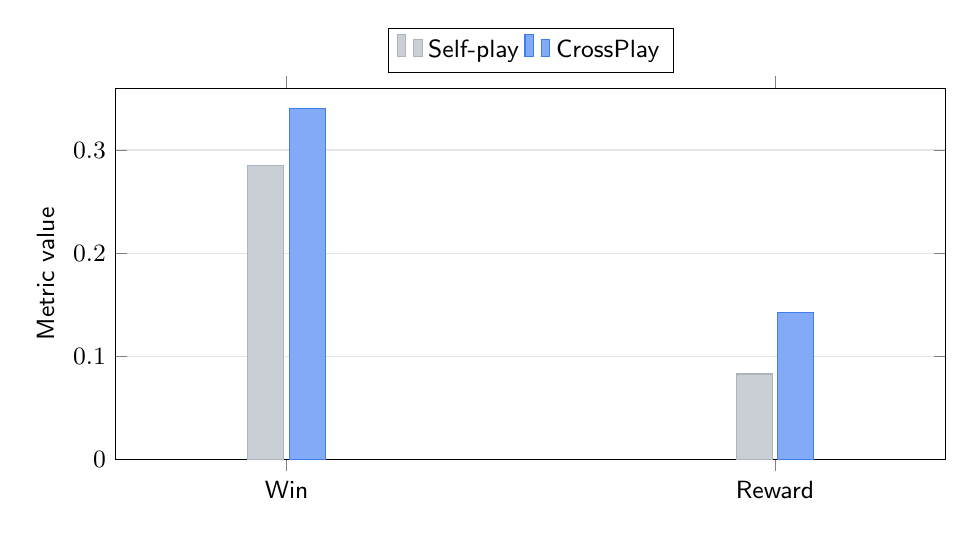
\begin{tikzpicture}
\begin{axis}[
  width=\linewidth,
  height=63mm,
  ybar,
  bar width=13pt,
  ymin=0,
  ymax=0.36,
  symbolic x coords={Win,Reward},
  xtick=data,
  ylabel={Metric value},
  tick label style={font=\small},
  ylabel style={font=\small},
  legend style={font=\small,at={(0.5,1.04)},anchor=south,legend columns=2},
  ymajorgrids=true,
  grid style={linegray!35},
  enlarge x limits=0.35
]
\addplot+[fill=linegray!65,draw=linegray] coordinates {(Win,\selfQwenWin) (Reward,\selfQwenReward)};
\addplot+[fill=dmblue!65,draw=dmblue] coordinates {(Win,\crossAWin) (Reward,\crossAReward)};
\legend{Self-play,CrossPlay}
\end{axis}
\end{tikzpicture}

\vspace{0.3em}
\begin{tabular}{@{}lcc@{}}
\toprule
Metric & Self-play & CrossPlay \\
\midrule
Win rate & \selfQwenWin & \crossAWin \\
Reward & \selfQwenReward & \crossAReward \\
\bottomrule
\end{tabular}
\end{minipage}
\hfill
\begin{minipage}[t]{0.32\linewidth}
\PanelTitle{3. SmolLM self-play}
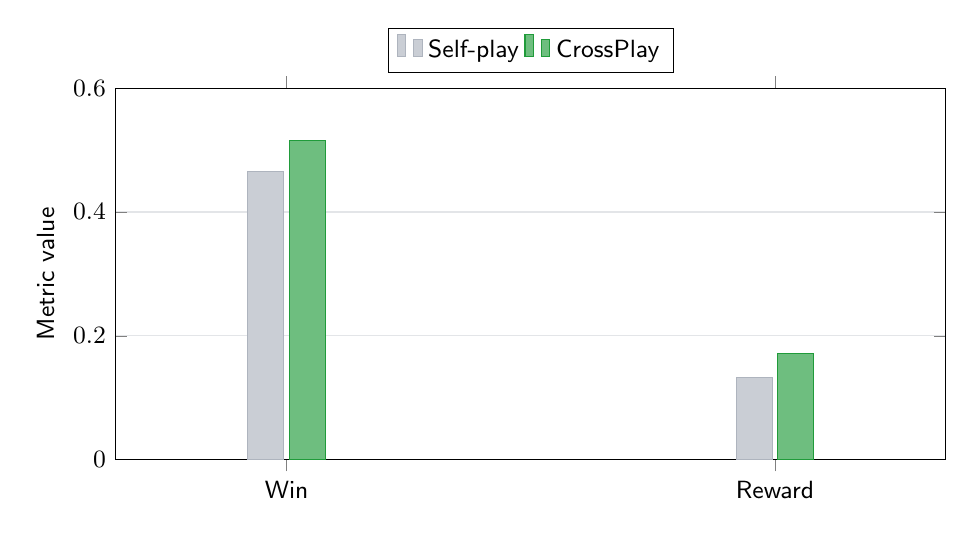
\begin{tikzpicture}
\begin{axis}[
  width=\linewidth,
  height=63mm,
  ybar,
  bar width=13pt,
  ymin=0,
  ymax=0.60,
  symbolic x coords={Win,Reward},
  xtick=data,
  ylabel={Metric value},
  tick label style={font=\small},
  ylabel style={font=\small},
  legend style={font=\small,at={(0.5,1.04)},anchor=south,legend columns=2},
  ymajorgrids=true,
  grid style={linegray!35},
  enlarge x limits=0.35
]
\addplot+[fill=linegray!65,draw=linegray] coordinates {(Win,\selfSmolWin) (Reward,\selfSmolReward)};
\addplot+[fill=goodgreen!65,draw=goodgreen] coordinates {(Win,\crossBWin) (Reward,\crossBReward)};
\legend{Self-play,CrossPlay}
\end{axis}
\end{tikzpicture}

\vspace{0.3em}
\begin{tabular}{@{}lcc@{}}
\toprule
Metric & Self-play & CrossPlay \\
\midrule
Win rate & \selfSmolWin & \crossBWin \\
Reward & \selfSmolReward & \crossBReward \\
\bottomrule
\end{tabular}
\end{minipage}

\end{document}
